\chapter{ROC曲线补充说明}\label{chapter:append1}
\begin{figure}[h]
	\centering
	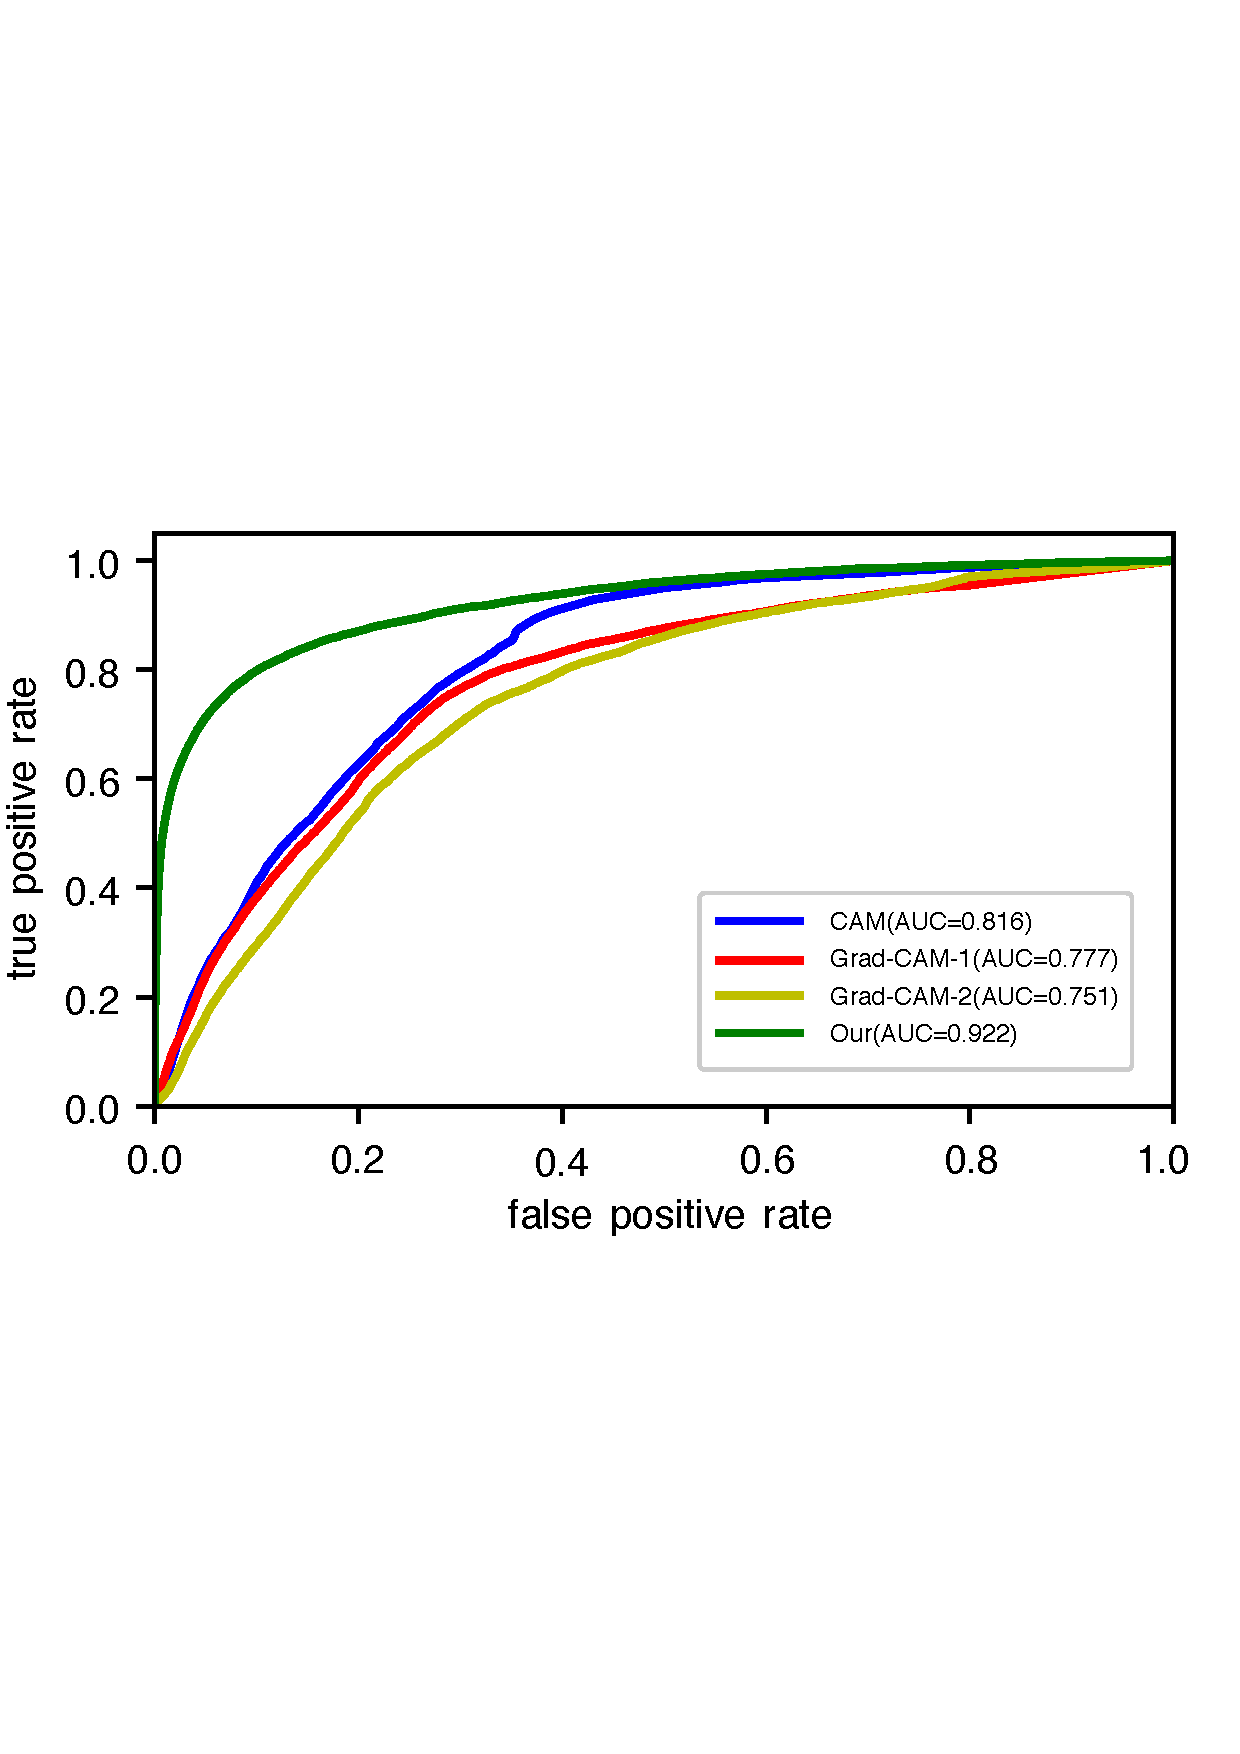
\includegraphics[width=0.98\textwidth]{figure/ROC_cam_grad_cam_our_diabetic_retinopathy}
	\caption{CAM、Grad-CAM和本文提出的模型根据二类视网膜糖尿病病变数据集绘制的ROC曲线。ROC曲线是根据数据集中$40$张像素级标注图像绘制。在ROC曲线产生之前,先将各种方法的定位结果的热图归一化到$[0, 1]$。根据P-R曲线及其AUC,与CAM、Grad-CAM相比,本文提出的模型性能表现最佳(AUC最高为$0.922$)。} 
	\label{fig:roc_cam_grad_cam_our_diabetic_retinopathy}
\end{figure}
\vspace{-1cm}
\begin{figure}[h]
	\centering
	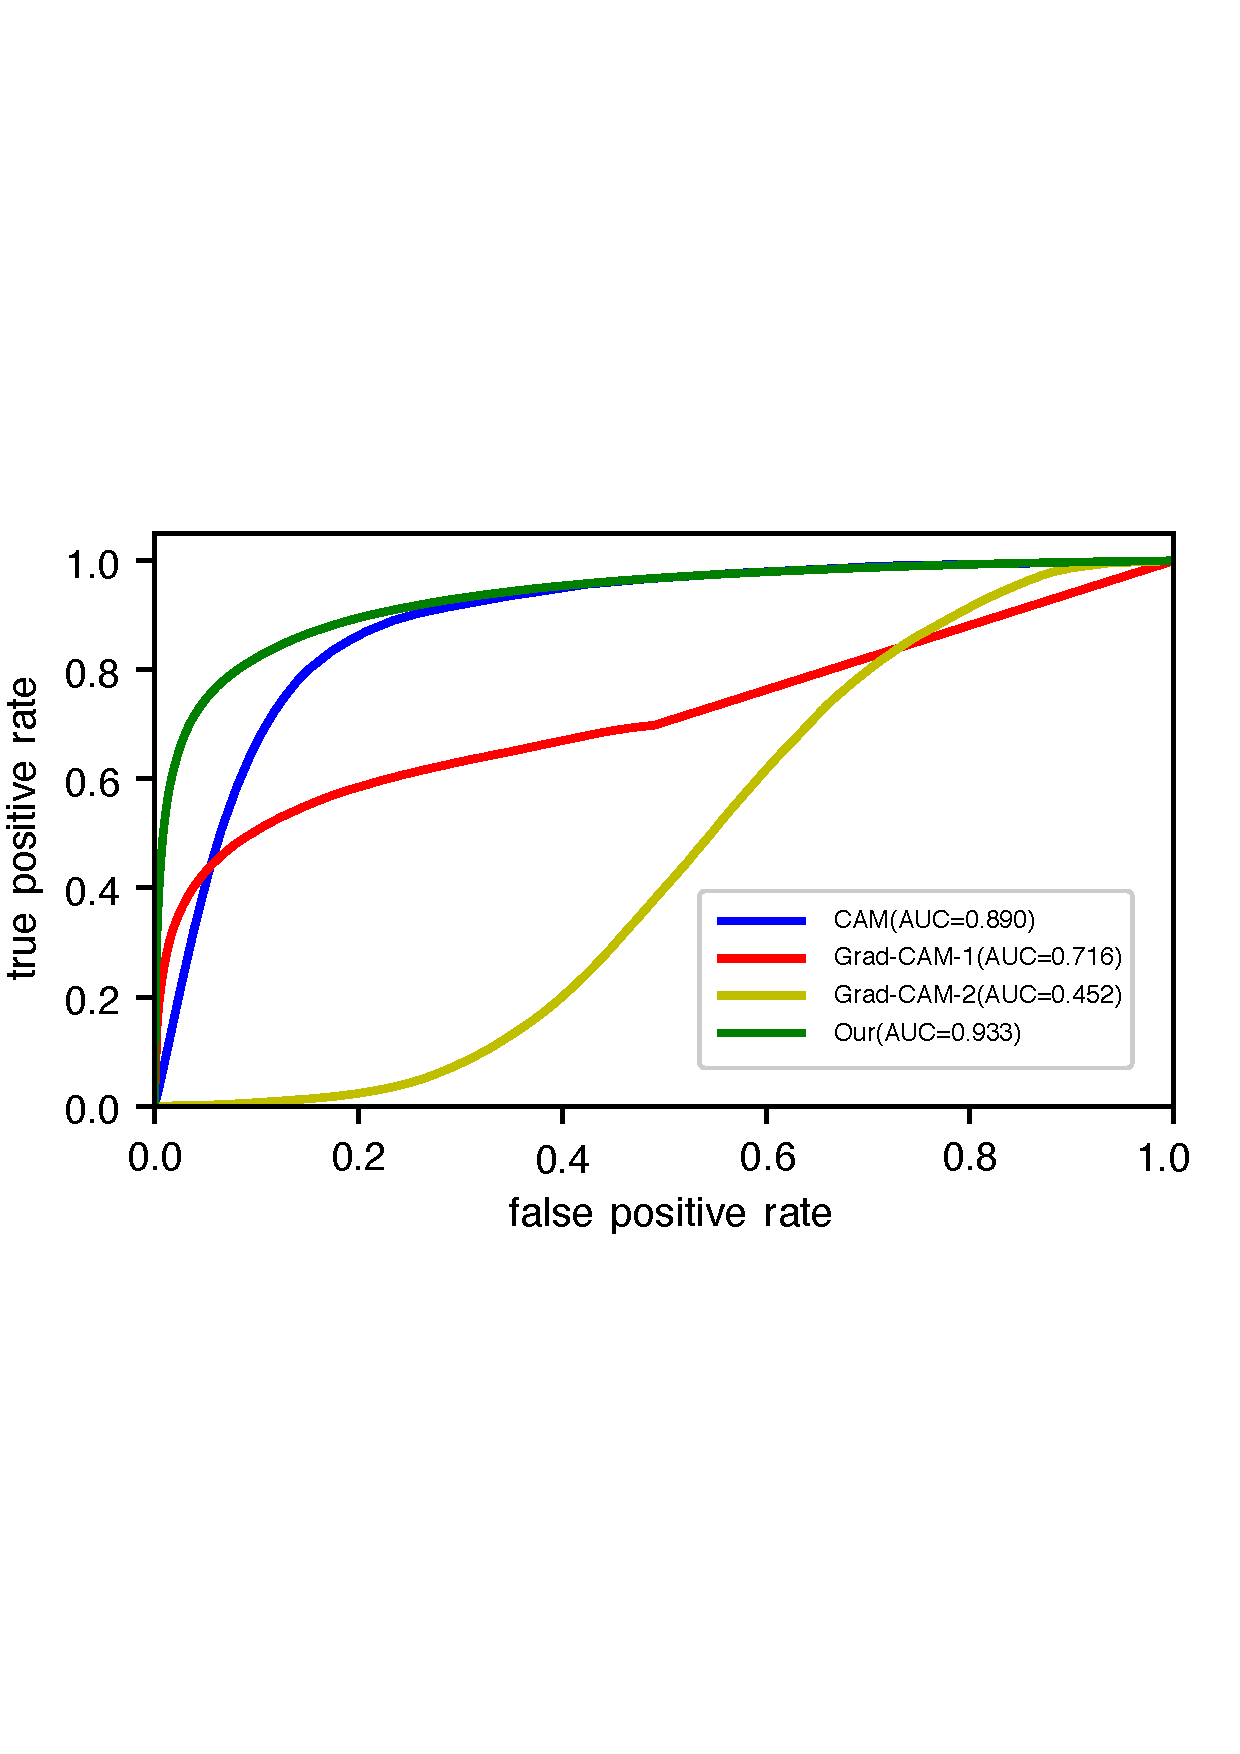
\includegraphics[width=0.98\textwidth]{figure/ROC_cam_grad_cam_our_simulated_skin_datasets}
	\caption{CAM、Grad-CAM和本文提出的模型根据二类模拟皮肤病病变数据集绘制的ROC曲线。ROC曲线是根据数据集中所有具有像素级标注的图像绘制。在ROC曲线产生之前,先将各种方法的定位结果的热图归一化到$[0, 1]$。根据P-R曲线及其AUC,与CAM、Grad-CAM相比,本文提出的模型性能表现最佳(AUC最高为$0.933$)。} 
	\label{fig:roc_cam_grad_cam_our_simulated_skin_datasets}
\end{figure}
\vspace{-1cm}
\begin{figure}[h]
	\centering
	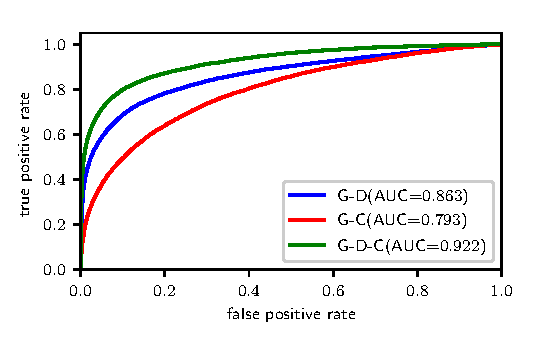
\includegraphics[width=0.98\textwidth]{figure/ROC_u_d_u_c_u_d_c_components}
	\caption{G-D模型、G-C模型和G-D-C模型根据二类视网膜糖尿病病变数据集中标注的部分图像绘制的P-R曲线。G-D-C模型本文提出的完整模型,G-D模型和G-C模型分别表示移去G-D-C模型中的CNN分类器模块和判别器模块得到的子模型。在ROC曲线产生之前,先将各种方法的定位结果的热图归一化到$[0, 1]$。P-R曲线及其AUC表明,与G-D模型和G-C模型相比,G-D-C模型的性能表现最佳(AUC最高为$0.922$)。}
	\label{fig:roc_u_d_u_c_u_d_c_components}
\end{figure}

\endinput
